\documentclass[sigconf,screen]{acmart}

%% Shared macros and notation of the paper.
\usepackage{amsmath}
\usepackage{stmaryrd}
\usepackage{booktabs}
\usepackage{xspace}
\usepackage{listings}
\usepackage{xcolor}
\usepackage{array}
\usepackage{pifont}
\usepackage{tikz}
\usetikzlibrary{arrows.meta,positioning,calc,fit,backgrounds}
\DeclareRobustCommand{\circled}[1]{\tikz[baseline=(c.base)]\node[circle,draw,inner sep=0.7pt,font=\tiny\bfseries] (c) {#1};}

% ---- names ----
\newcommand{\tool}{\textsc{Arbor}\xspace}   % our fuzzer
\newcommand{\pg}{PostgreSQL\xspace}
\newcommand{\pgg}{\texttt{.pgg}\xspace}       % our typed grammar format
\newcommand{\gate}{validation gate\xspace}
\newcommand{\arm}[1]{\textsf{#1}\xspace}      % an evaluated configuration (arm)

% ---- notation (one macro per symbol; comment says what it means) ----
\newcommand{\Q}{\ensuremath{Q}\xspace}                     % a generated query
\newcommand{\Tree}[1]{\ensuremath{T(#1)}}                     % derivation tree of a query
\newcommand{\Res}[1]{\ensuremath{\llbracket #1 \rrbracket}}   % result multiset of a query
\newcommand{\Part}[2]{\ensuremath{#1[#2]}}                    % query with predicate p at a node replaced

% ---- research questions ----
\newcommand{\rqref}[1]{\textbf{RQ#1}\xspace}

% ---- results: one boxed, numbered claim per observation ----
\newcounter{observation}
\newsavebox{\obsbox}
\newenvironment{observation}
  {\refstepcounter{observation}\par\smallskip\noindent\begin{lrbox}{\obsbox}\begin{minipage}{0.95\linewidth}\textbf{Observation~\theobservation.}~}
  {\end{minipage}\end{lrbox}\fbox{\usebox{\obsbox}}\par\smallskip}

% ---- symbols ----
\newcommand{\cmark}{\ding{51}}
\newcommand{\xmark}{\ding{55}}

\lstset{basicstyle=\ttfamily\footnotesize,columns=fullflexible,
        keepspaces=true,frame=single,framesep=2pt,xleftmargin=4pt,
        numbers=left,numberstyle=\tiny,numbersep=4pt}

% long \texttt words otherwise run into the margin
\setlength{\emergencystretch}{3em}


\setcopyright{none}
\settopmatter{printacmref=false}
\renewcommand\footnotetextcopyrightpermission[1]{}
\acmDOI{}
\acmISBN{}
\acmConference[CS-5187 Term Project]{CS-5187 Term Project, IIT Guwahati}{November 2026}{Guwahati, India}
\acmYear{2026}
\citestyle{acmauthoryear}

\begin{document}

\title[Check the Tree]{Check the Tree: Finding Wrong Results in PostgreSQL with Typed Derivation Trees and Commit-Directed Grammar Extension}

\author{Venu Kummari}
\email{v.kummari@iitg.ac.in}
\affiliation{\institution{Indian Institute of Technology Guwahati}\city{Guwahati}\country{India}}
\author{Bhuvan Chilukuti}
\email{c.bhuvan@iitg.ac.in}
\affiliation{\institution{Indian Institute of Technology Guwahati}\city{Guwahati}\country{India}}
\author{Gowtham Reddy}
\email{r.doma@iitg.ac.in}
\affiliation{\institution{Indian Institute of Technology Guwahati}\city{Guwahati}\country{India}}
\renewcommand{\shortauthors}{Kummari, Chilukuti, and Reddy}

\begin{abstract}
When a database system returns a wrong result, nothing tells the user: there is
no error, no crash and nothing in the logs. Most fuzzers for \pg look for
crashes, and the oracles that can detect wrong results are tied to small query
generators of their own. As an example, \pg~17, 18 and master answer
\texttt{true} for \texttt{'(,)'::int4range @> NULL}, although a strict operator
must return NULL. We also found that of 23 recent query-processing fixes in \pg
master, 20 change what a query returns, but only 9 of them crash or raise an
internal error. This paper presents \tool, a fuzzer that keeps every generated
query as a typed derivation tree. Because the tree is kept, metamorphic oracles
such as TLP, NoREC, expression rewrites, CTE and table fences and a row-level
security check can rewrite a single node of known type at any level of the
query. Triage then reduces a failure on the same tree. Plan variants and the last release
of \pg act as two more oracles. In addition, an LLM reads recent commits and
proposes grammar alternatives and equivalence rewrites, and a validation gate
accepts them only if the server runs them, they reach the changed lines and no
rewrite changes a result. In five one-hour trials per configuration, the typed
grammar covers 36.7\% of backend lines against 22.2\% for random mutation, and
the oracles double the number of plan shapes reached. We reported ten bugs found
with \tool; eight are fixed upstream, six of them with our patches, and \tool
rediscovers all ten in one 150-second run. Of 93 triaged candidates, 8 are real
and 15 are duplicates of real bugs, and the false positives come from a few
classes that we fixed. The LLM adds SQL features but no coverage, and one
rewrite it proposed passed our gate although it is not an identity. On a
benchmark of 23 real bugs, the best configuration found 2 of 20. Our main lesson
is that oracle precision, not generator reach, is what limits a wrong-result
fuzzer. Finally, with per-engine dialect overlays and optimizer-rule feedback,
\tool also tests DuckDB, SQLite, Turso and DataFusion, where it found five more
bugs that we reported upstream with fixes.

\end{abstract}

\begin{CCSXML}
<ccs2012>
  <concept>
    <concept_id>10011007.10011074.10011099.10011102.10011103</concept_id>
    <concept_desc>Software and its engineering~Software testing and debugging</concept_desc>
    <concept_significance>500</concept_significance>
  </concept>
  <concept>
    <concept_id>10002951.10002952</concept_id>
    <concept_desc>Information systems~Data management systems</concept_desc>
    <concept_significance>300</concept_significance>
  </concept>
</ccs2012>
\end{CCSXML}
\ccsdesc[500]{Software and its engineering~Software testing and debugging}
\ccsdesc[300]{Information systems~Data management systems}

\keywords{fuzzing, database testing, test oracles, metamorphic testing,
  grammar-based testing, large language models, PostgreSQL}

\maketitle

\section{Introduction}
\label{sec:intro}

Imagine running a reporting query on \pg and getting back a row that should not
be there. The query does not crash, no error is raised, and the server log looks
normal. Nothing tells you that the answer is wrong. This kind of failure, a
\emph{wrong result}, is in our view the most harmful bug a database system can
have, because the user has no way to notice it.

Most fuzzers for database systems look for crashes instead.
SQLsmith~\cite{sqlsmith} generates random queries from the system catalog, and
SQUIRREL~\cite{zhong2020squirrel} mutates SQL with coverage feedback; both
report a bug when the server crashes or an assertion fails. To catch a wrong
result, a fuzzer needs a \emph{test oracle}, something that knows what the
right answer is. Differential testing compares two systems on the same
query~\cite{slutz1998rags}. Metamorphic oracles such as Ternary Logic
Partitioning (TLP)~\cite{rigger2020tlp}, NoREC~\cite{rigger2020norec} and
equivalent expression transformation~\cite{jiang2024eet} instead compare a query
with a rewritten version that must return the same rows. These oracles rewrite
the SQL text, so each tool comes with its own small query generator whose output
the oracle understands. This leaves a gap. Grammar-based generators reach deep
into the planner but do not know which parts of a query can be rewritten safely,
while oracle-based tools know how to rewrite but cover only a small part of SQL.
Neither of them knows what changed in the code recently, even though the \pg
planner changes every week and most new bugs live in the newest code.

Figure~\ref{fig:motivating} shows a real wrong result that \tool found. Since
\pg~17, the planner replaces \texttt{range @> elem} with the constant
\texttt{true} when the range is unbounded on both sides, and with \texttt{false}
when the range is empty. The operator is strict, so for a NULL element the
correct answer is NULL. The folded constant gives a wrong answer under
\texttt{NOT}, in \texttt{IS NULL} tests, in \texttt{CASE} expressions and in
outer joins, where unmatched rows carry NULLs. We reproduced the bug on release
18.6 and on master. \tool found it with a typed rewrite of the derivation tree,
by wrapping the range in a scalar subquery, within the first 150 test cases that
used this rewrite. The example is not an isolated case: when we put back 23
recent fixes from \pg master (Section~\ref{sec:rq3}), 20 of them changed what a
query returns, and only 9 could be seen by a fuzzer that only watches for
crashes. The closest previous work is query plan guidance~\cite{ba2023qpg},
which steers a generator toward new plan shapes using SQLancer's oracles, and
Fuzz4All~\cite{xia2024fuzz4all}, which uses a large language model (LLM) as the
generator. Neither connects the generator to the code that changed.

\begin{figure}[t]
\begin{lstlisting}[numbers=none,escapechar=!,language=SQL]
SELECT c,
       '(,)'::int4range @> c AS contains,
         -- must be NULL when c is NULL
       NOT ('empty'::int4range @> c) AS not_empty
         -- must be NULL when c is NULL
FROM (VALUES (NULL::int), (1)) v(c);

  c   | contains | not_empty
------+----------+----------
 NULL | t        | t          !\textbf{$\leftarrow$ wrong: the planner folded the call to a constant}!
 1    | t        | t
\end{lstlisting}
\caption{A wrong result in \pg~17, 18.6 and master that \tool found. The
planner support function for range containment returns \texttt{true} or
\texttt{false} for a NULL element, where the strict operator gives NULL. No
error or crash reveals it; only an oracle that compares two equivalent queries
does.}
\label{fig:motivating}
\end{figure}

To close this gap we built \tool, a grammar-aware fuzzer for \pg based on three
ideas. First, a \emph{typed grammar} generates SQL as derivation trees in which
every node knows its type and its place in the query
(Section~\ref{sec:grammar}). Second, the oracles work on the tree rather than on
the text: TLP and NoREC can be applied at any query level, alongside typed
expression rewrites, a row-level security check, and plan-variant and
cross-version oracles (Section~\ref{sec:oracles}). Third, the grammar is
extended from recent commits: an LLM reads a commit and proposes grammar
alternatives, seed queries and new equivalence rewrites, and a \gate accepts
them only if the server runs them, they execute the lines the commit changed,
and no rewrite changes a result (Section~\ref{sec:llm}). Around these ideas,
\tool reduces every finding on its derivation tree and its tokens, localizes a
wrong result to a planner path or to a rewrite that is always applied, and drafts
the upstream report (Section~\ref{sec:triage}).

We evaluated \tool on \pg master. The typed grammar reaches 36.7\% of backend
lines in an hour against 22.2\% for random mutation, with 99\% valid statements
against 26\% (\rqref{1}), and the oracles double the number of distinct plan
shapes. We reported ten bugs found with \tool, eight of which are fixed
upstream, six with our patches, and \tool rediscovers all ten in one
150-second run (\rqref{2}). Of 93 triaged candidates, 8 are real and 15 are
duplicates of real bugs, and the false positives come from a small number of
classes. On a benchmark of 23 re-injected bugs, no configuration found more
than 2 of 20 in one hour (\rqref{3}). The LLM extension adds SQL features but no
coverage, and the gate accepted one rewrite that is not an identity
(\rqref{4}). What we learned is that oracle precision, not generator power,
limits a wrong-result fuzzer: a generator that reaches more of SQL also reaches
more of the corner cases where two ``equivalent'' queries are in fact not
equivalent.

In summary, this paper makes the following contributions:
\begin{itemize}
  \item a typed \pg grammar whose derivation trees are used for generation,
    mutation, metamorphic rewriting and reduction (Section~\ref{sec:approach});
  \item tree-based oracles, together with the measured precision of each
    (Section~\ref{sec:rq2});
  \item a commit-directed LLM extension with a \gate that tests proposed
    rewrites on values and on queries (Section~\ref{sec:llm});
  \item a benchmark of 23 real \pg bugs put back into one server
    (Section~\ref{sec:rq3}); and
  \item ten reported \pg bugs, eight of them fixed upstream (six with our
    patches), released together with the tool and all data
    (Section~\ref{sec:data}).
\end{itemize}
The rest of the paper defines the problem (Section~\ref{sec:problem}), describes
the approach and its implementation (Sections~\ref{sec:approach}
and~\ref{sec:impl}), and then reports the evaluation (Section~\ref{sec:eval}).

\section{Problem Statement}
\label{sec:problem}

Before describing \tool, we fix the terms we use in the rest of the paper. Let
$G$ be a typed grammar for the SQL dialect of \pg and $S$ a database schema. A
\emph{test case} is a sequence of statements derived from $G$ over $S$ and run
in one transaction that is rolled back at the end. The \emph{derivation tree}
\Tree{\Q} of a query \Q records which alternative each rule took, and its leaves,
read from left to right, give the text of \Q. A query has a \emph{wrong result}
when the server returns, without any error, a multiset \Res{\Q} that differs
from what the SQL standard and the \pg documentation define. An \emph{oracle}
looks at the server's response to a test case and decides between \emph{pass}
and \emph{bug candidate}. A metamorphic oracle such as TLP~\cite{rigger2020tlp}
or NoREC~\cite{rigger2020norec} compares \Q with a rewritten query. Similarly,
a \emph{plan variant}, the same query run under a setting such as
\texttt{SET enable\_hashjoin = off}, must return the same multiset as the
original.

\paragraph{Sound rewrites.} A tree rewrite $r$ maps \Tree{\Q} to a second tree.
We call it \emph{sound} for \Q if $\Res{\Q} = \Res{r(\Q)}$ holds on every correct
server. Some rewrites are sound only under conditions, for example only if no
\texttt{LIMIT} without \texttt{ORDER BY} appears below the rewritten node, and
these conditions must be checked on the tree before the rewrite is applied. An
unsound rewrite produces \emph{false positives}, that is, candidates that are
not bugs.

\paragraph{Goal.} Given a fixed time budget $B$ and one server, we want to find
as many distinct bugs as possible, where a bug is a crash, a failed assertion,
an internal error (SQLSTATE class \texttt{XX}) or a wrong result. At the same
time, we want the \emph{precision} of each oracle to stay high:
\begin{equation}
  \mathit{precision}(o) = \frac{|R_o|}{|R_o| + |F_o|}
  \label{eq:precision}
\end{equation}
Here $R_o$ and $F_o$ are the real bugs and the false positives among the
distinct candidates reported by oracle $o$, after de-duplication by signature
(Section~\ref{sec:triage}). Candidates that do not reproduce (flaky ones) are
counted separately. A duplicate of a bug that was already reported upstream is
still a real bug, so we also give the precision with duplicates counted in
$R_o$.

\paragraph{Why not let an LLM write the test cases?} An LLM can write SQL that
targets a specific feature, but it needs a few seconds per call. In an hour it
produces at most a few thousand test cases, while the grammar arm produced
71{,}228 in the same time (Table~\ref{tab:rq1}). Queries written by an LLM are also not
derivation trees, so the tree-based oracles cannot rewrite them. For these
reasons we use the LLM to \emph{extend the grammar} instead: a few calls per
commit, after which the grammar generates thousands of variations on its own.

\section{Approach}
\label{sec:approach}

Figure~\ref{fig:overview} gives an overview of \tool. The central idea is to
keep every generated query as a typed derivation tree until it has been run, so
that the oracles can rewrite a single node whose type and position are known,
instead of editing SQL text. In \tool the same tree is used for four things:
generation builds it, mutation re-derives one subtree, the oracles rewrite one
typed node, and triage shrinks it by replacing subtrees with their smallest
derivation. The fuzzing loop (Steps 1--4) runs thousands of test cases per
minute, while the LLM loop (Step 5) runs only a few times per commit, before a
campaign starts. We describe the steps in order.

\begin{figure*}[t]
  \centering
  %% Overview of Arbor. Steps match the subsections of Section 4.
%% Grayscale-safe (black lines, black!6 fill), \scriptsize text.
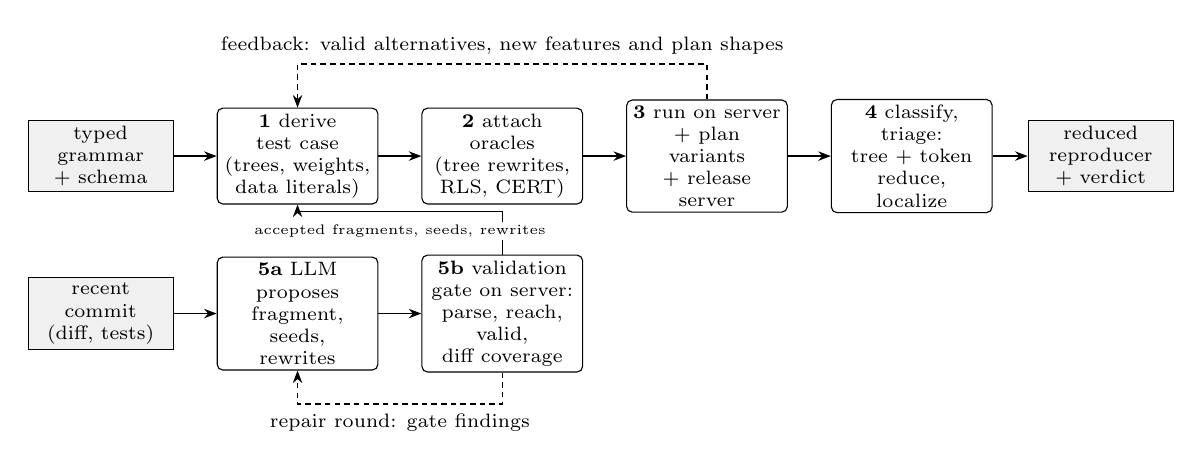
\begin{tikzpicture}[
    x=1cm, y=1cm, font=\scriptsize,
    box/.style={draw, rounded corners=2pt, align=center, inner sep=2pt,
                minimum height=10mm, text width=19mm, fill=white},
    io/.style={draw, align=center, inner sep=2pt, fill=black!6, text width=17mm, minimum height=8mm},
    flow/.style={-{Stealth[length=1.6mm]}, line width=0.5pt},
    back/.style={-{Stealth[length=1.6mm]}, line width=0.5pt, dash pattern=on 2pt off 1.5pt},
  ]
  % top row: the fuzzing loop
  \node[io]  (g)  at (0,0)    {typed grammar\\+ schema};
  \node[box] (s1) at (2.5,0)  {\textbf{1} derive test case\\(trees, weights,\\data literals)};
  \node[box] (s2) at (5.1,0)  {\textbf{2} attach oracles\\(tree rewrites,\\RLS, CERT)};
  \node[box] (s3) at (7.7,0)  {\textbf{3} run on server\\+ plan variants\\+ release server};
  \node[box] (s4) at (10.3,0) {\textbf{4} classify, triage:\\tree + token reduce,\\localize};
  \node[io]  (out) at (12.7,0) {reduced\\reproducer\\+ verdict};
  % bottom row: the LLM loop
  \node[io]  (c)  at (0,-2.0)   {recent commit\\(diff, tests)};
  \node[box] (s5) at (2.5,-2.0) {\textbf{5a} LLM proposes\\fragment, seeds,\\rewrites};
  \node[box] (s6) at (5.1,-2.0) {\textbf{5b} \gate on server:\\parse, reach, valid,\\diff coverage};
  \draw[flow] (g) -- (s1);
  \draw[flow] (s1) -- (s2);
  \draw[flow] (s2) -- (s3);
  \draw[flow] (s3) -- (s4);
  \draw[flow] (s4) -- (out);
  \draw[back] (s3.north) -- ++(0,0.45) -| node[pos=0.25, above] {feedback: valid alternatives, new features and plan shapes} (s1.north);
  \draw[flow] (c) -- (s5);
  \draw[flow] (s5) -- (s6);
  \draw[back] (s6.south) -- ++(0,-0.4) -| node[pos=0.25, below] {repair round: gate findings} (s5.south);
  \draw[flow] (s6.north) -- ++(0,0.55) -| (s1.south);
  \node[font=\tiny, fill=white, inner sep=1pt] at (3.8,-0.95) {accepted fragments, seeds, rewrites};
\end{tikzpicture}

  \caption{Overview of \tool. The top row is the fuzzing loop: test cases are
  derived from the typed grammar, oracles are attached as rewrites of the
  derivation tree, and the server runs each query under several settings.
  The bottom row runs before a campaign: an LLM turns a recent commit into
  grammar alternatives, and the \gate accepts them only when the server runs
  them and they reach the changed lines.}
  \label{fig:overview}
\end{figure*}

\subsection{Step 1: Derive Test Cases from a Typed Grammar}
\label{sec:grammar}

We wrote a grammar for the SQL that \pg~18 and master accept, using a small
format of our own (\pgg). In the campaigns it had 78 rules with 421 alternatives
over 13 SQL types; after the additions for the rediscovery runs
(Section~\ref{sec:rq2}) it has 83 rules and 437 alternatives. A rule can be
parameterised by a type, as in \texttt{expr<T>}, so a derivation only combines
expressions that type-check. Weights decide how often each alternative is
chosen. Some things cannot be expressed in a context-free grammar, and for these
we use \emph{builtins} written in Python: \texttt{@col(T)} picks a visible column
of type $T$ in the current scope, \texttt{@table} binds a fresh alias, and
\texttt{@group\_keys} turns the current query level into a grouped one, after
which only grouped columns and aggregates are visible. The schema has 9
relations, with partitions, inheritance, a view, indexes of four access methods
and NULLs in most columns.

A test case consists of up to two setup statements (DDL, DML, \texttt{ANALYZE},
or \texttt{SET LOCAL} of a planner setting) followed by one or two queries.
During derivation, the engine wraps the tokens of every node in invisible
markers, so that after rendering it knows the exact token span of each node.
Half of the test cases are fresh derivations; the other half take a test case
from the corpus and re-derive one of its subtrees. A test case is added to the
corpus when it produces a new bug signature, a new SQL feature, a new pair of
features, or a new plan shape. A plan shape is a digest of the node types in the
\texttt{EXPLAIN} output~\cite{ba2023qpg}.

\paragraph{Feedback and data.} Each alternative has a multiplicative weight
that grows when a test case using it enters the corpus and shrinks when its
statement fails (rate $\eta=0.1$, bounded to $[0.2,5]$). Some literals are taken
from a \emph{data profile}, which contains the minimum, maximum and quantiles of
every column together with edge values of each type, such as $-0$, NaN,
$\pm$Infinity and the empty array. This way, generated predicates select a
real share of the rows. Grammar-based generation itself is not new; what the
later steps need from it are the types, the scoping builtins and the node
spans.

\subsection{Step 2: Attach Oracles as Tree Rewrites}
\label{sec:oracles}

Once a query is derived, \tool picks at most one metamorphic check for it and
stores it with the test case as a pair of queries that must return the same
multiset. All of these checks are built on the derivation tree.

\paragraph{Partitioning and counting.} \emph{TLP on \texttt{WHERE}} chooses a
\texttt{SELECT} whose result is used as a multiset, which can be the query
itself, a derived table, a CTE body, an arm of a set operation, or an
\texttt{IN}, \texttt{EXISTS} or \texttt{LATERAL} subquery. It then splits its
\texttt{WHERE p} into $p$, \texttt{NOT p} and \texttt{p IS NULL} and combines the
three parts with \texttt{UNION ALL}. Since the rewrite edits one node, it also
works inside nested queries, where text-based TLP cannot be applied. \emph{TLP
on \texttt{HAVING}} works the same way, except that the unpartitioned side keeps
\texttt{HAVING TRUE}: without \texttt{GROUP BY}, it is the \texttt{HAVING} clause
that makes a level a single-group aggregate. \emph{TLP on aggregates} checks
that a global \texttt{MIN}, \texttt{MAX}, \texttt{SUM}, \texttt{COUNT},
\texttt{BIT\_*} or \texttt{BOOL\_*} equals its combination over the three
partitions, for example the \texttt{MIN} of the \texttt{MIN}s or the
\texttt{SUM} of the \texttt{COUNT}s. \emph{NoREC} compares \texttt{count(*)}
with \texttt{WHERE p} against the sum of \texttt{CASE WHEN p THEN 1 ELSE 0 END}.

\paragraph{Equivalent forms of one node.} \emph{Expression rewrites} replace one
typed expression $e$ with an equivalent form: \texttt{COALESCE(e,e)},
\texttt{(SELECT e)} or \texttt{CASE WHEN TRUE THEN e END} for any type; $e+0$ or
$e \cdot 1$ for numbers; \texttt{e || ''} for text; and \texttt{NOT NOT p},
\texttt{p AND TRUE} or \texttt{p OR FALSE} for predicates. \emph{Predicate
rewrites} turn \texttt{x IN (a, b)} into \texttt{(x = a) OR (x = b)}, which
\pg~18 converts back into \texttt{= ANY}; they also turn \texttt{a < b} into
\texttt{NOT (a >= b)}, which three-valued logic keeps exact, and
\texttt{BETWEEN} into two comparisons. The \emph{NOT NULL conjunct} rewrite turns
\texttt{WHERE p} into \texttt{WHERE p AND c IS NOT NULL} for a NOT NULL column
$c$ that $p$ uses, to exercise the planner's NOT NULL simplifications; it is
skipped under outer joins and for generated columns, where such a column can
still be NULL. Finally, \emph{ORDER BY removal} drops the statement's own
\texttt{ORDER BY}, and \emph{CTE materialisation} toggles
\texttt{MATERIALIZED}. The \emph{table fence} turns one table reference into
\texttt{(SELECT * FROM t OFFSET 0)}, which prevents the planner from pushing
predicates into it, removing it, or pruning its partitions.

\paragraph{Security and estimates.} For \emph{row-level security}, five tables
have a policy, defined in one file that both the server and the rewrite use. The
query runs once as a restricted role, under the policies, and once as a
superuser with every protected table $t$ replaced by \texttt{(SELECT * FROM t
WHERE \textit{policy})}. If the two results differ, the policies either let a
row through or hide a row they should not. Following CERT~\cite{ba2024cert},
adding a \texttt{WHERE} clause to a query must not increase the planner's row
estimate; this check compares the \texttt{EXPLAIN} estimates, and a violation is
reported as a \emph{performance} candidate, separately from bugs.

In every case, a check is attached only if its rewrite is sound for that query
(Section~\ref{sec:problem}).

\subsection{Step 3: Run the Test Case Several Ways}
\label{sec:run}

The server runs each test case inside a transaction, with one savepoint per
statement, and rolls it back at the end, so test cases cannot affect each other.
For each deterministic query, \tool runs three extra things: (i)~both sides of
the attached check; (ii)~the query under two of 18 \emph{plan variants}, chosen
at random per query, such as hash join only, no hash aggregation, forced
parallel plans, partitionwise join, no eager aggregation, or JIT; and (iii)~the
whole test case on a server of the last release, \pg~18.6, with a separate
database for each worker (the \emph{cross-version oracle}). Results are compared
as order-insensitive digests. The digests ignore differences that no plan
controls: trailing zeros of equal \texttt{numeric} values, the sign of a float
zero, the last digits of finite floats in aggregates, and the text of equal
\texttt{interval} values.

\subsection{Step 4: Classify, De-duplicate, Triage}
\label{sec:triage}

The oracle looks at the statement results and at the server log. A
\texttt{TRAP} line means an assertion failure, a lost connection without one
means a crash, an error of class \texttt{XX} is an internal error, and a
confirmed mismatch of any digest is a wrong result. A metamorphic mismatch
counts only if it repeats when both sides are run again, and crash evidence
counts only if it carries the process id of the test case's own backend or its
parallel workers. Each candidate gets a \emph{signature}, which is the assertion
location, the normalised backtrace or error message, or, for wrong results, the
oracle and the shape of the query. Only the first test case with a given
signature is saved.

Triage then reproduces the candidate three times on a fresh connection and
reduces it in two stages. \emph{Tree reduction} works on the derivation trees
that the grammar arm stores with every failure. It drops a statement, drops one
repetition, or replaces a subtree with the smallest derivation of the same rule
and type, and replays the trees through the generator, which re-binds names,
aliases and types. As a result, every candidate is valid SQL, and the server's
time is spent only on checking whether the failure is still there. \emph{Token
reduction} comes next: delta debugging~\cite{zeller2002dd} removes statements,
then clauses, list items and parenthesised groups level by level over the
parenthesis tree~\cite{misherghi2006hdd}, and finally single tokens. A step is
kept only if the same failure still occurs, meaning the same assertion, the same
normalised message, or the same oracle and plan variant. For a metamorphic
candidate, the two queries are reduced together so that they stay a valid pair.

\paragraph{Localization.} For a reduced wrong result, \tool runs the queries
under every plan variant. If some variant removes the disagreement, the bug is
in the code path that this setting switches, and the report names the setting
and its source files. If no variant helps, the cause is a rewrite that is always
applied, constant folding, a planner support function, or expression evaluation.
The output of triage is a short reproducer, the rows each side returned, the
localization and a draft report in the format of the \pg bug form.

\subsection{Step 5: Extend the Grammar from Recent Commits}
\label{sec:llm}

The last step connects the grammar to the code that changed. It has two parts.

\paragraph{Step 5a: propose.} \tool lists the commits of \pg master that change
the optimiser, the executor, the parser or SQL-callable functions and that add
regression tests. For each commit it builds a digest containing the commit
message, the changed functions, the SQL the commit added to the tests, and the
\emph{diff-coverage targets}, which are the changed lines of each C file. The
LLM receives this digest together with a fixed, cached system prompt that
describes the \pgg format, the builtins, the conventions of the grammar, the
schema and the whole current grammar. It answers with structured output: a
rationale, a fragment of new alternatives, one to five seed test cases, the
features it targets, and up to three \emph{equivalence rewrites}. An
equivalence rewrite is a template over one expression of a given type, such as
\texttt{CASE WHEN \{e\} IS NULL THEN NULL ELSE \{e\} END}, that the model claims
equals \texttt{\{e\}} for every value. The commit miner never shows the model a
fix that the benchmark of Section~\ref{sec:rq3} reverts.

\paragraph{Step 5b: validate.} No model output reaches a campaign unless the
server agrees with it. The \gate runs five checks in order: (i)~\emph{parse}:
the fragment parses with the grammar, adds no types and uses only known
builtins; (ii)~\emph{reachability}: in a sample of 150 test cases with the new
alternatives boosted, they are used at least five times; (iii)~\emph{validity}:
at least 60\% of the statements that use them run without error;
(iv)~\emph{seeds}: each seed runs; and (v)~\emph{diff coverage}: on a gcov build,
the sample executes more of the commit's changed lines than the same sample
without the fragment. When a check fails, its findings (the parse error, the
most frequent error messages, the uncovered lines) go back to the model for up
to three repair rounds. Every round is recorded in a ledger with its tokens,
cost and the gate's report.

A proposed rewrite is a claim about semantics, so the gate tests it twice.
First, the server evaluates \texttt{rewrite(v) IS NOT DISTINCT FROM v} for NULL,
the edge values of the type and quantiles of the data. Then \tool applies the
rewrite alone to the expressions of 150 test cases, with confirmation re-runs.
The rewrite is accepted only if no value and no query shows a difference, after
which it becomes one of the expression rewrites of Step~2. Neither test varies
the collation, so the gate also rejects any template with an explicit
\texttt{COLLATE} (Section~\ref{sec:rq4}).

\section{Implementation}
\label{sec:impl}

We implemented \tool in Python. It is about 11{,}000 lines of code with 151 unit
tests, plus the grammar, which had 628 lines in the campaigns and has 651 after
the additions described in Section~\ref{sec:rq2}. \tool talks to \pg through
\texttt{psycopg} and reads the server log to find evidence of assertion
failures and crashes. Every trial runs as a resumable process that writes its
events, timeline and failures as JSON, so an interrupted trial can continue
where it stopped. The code is split into six parts:
\begin{itemize}
  \item the \pgg parser and derivation engine, which handles scopes, type
    variables, node spans and the \texttt{MINIMAL} marker used by reduction;
  \item the generator, with the corpus, the alternative weights and the data
    profile;
  \item the executor, which manages savepoints and plan variants and runs the
    metamorphic, RLS and CERT checks, with a wrapper for the cross-version
    oracle;
  \item triage, covering reproduction, tree and token reduction, localization,
    report drafts, bisection and the precision ledger;
  \item the benchmark scripts, including \texttt{bench verify} and
    \texttt{bench attribute}; and
  \item the LLM arm, made of the commit miner, the prompts, a client that stores
    every response so that a run can be replayed, the \gate and the ledger.
\end{itemize}
A single configuration file selects the generator, the oracles and the budget of
a campaign, so every arm in the evaluation differs only in its configuration.

\section{Evaluation}
\label{sec:eval}

We ask four questions.
\begin{itemize}
  \item[\rqref{1}] Does the typed grammar reach more of \pg than a
    random-mutation generator in the same time: more valid statements, more
    covered lines and branches, more SQL features and plan shapes?
  \item[\rqref{2}] Which bugs does \tool find, and how precise is each oracle?
  \item[\rqref{3}] On real bugs put back into \pg, which configuration finds
    how many, and how fast?
  \item[\rqref{4}] What does the commit-directed LLM extension add, and what
    does it cost in tokens, money and repair rounds?
\end{itemize}

\subsection{Subject and Benchmark}
\label{sec:subjects}

All servers are built from \pg master \texttt{26bd08fb} (16~October~2026) with
assertions on. For \rqref{3} we built a benchmark in the style of
Magma~\cite{hazimeh2020magma} by reverting fixes: every commit between
31~July and 16~October~2026 that fixes a bug in the optimiser, executor,
parser, rewriter or a SQL-callable function, adds a regression test, and
reverts cleanly alone and together with the others, 23 in all. We build the
\emph{fixed} server, one \emph{solo} server per bug (only that fix reverted),
and the \emph{injected} server (all 23 reverted) on which the campaigns run.
A proof of concept (PoC) written from each regression test changes its result
for 20 bugs: 8 wrong results, 5 internal errors, 4 assertion failures, 2
missing errors and 1 wrong error. A crash-only fuzzer can see only the 9
assertions and internal errors. The other three change only the plan, or need an
equality operator that returns NULL for non-NULL inputs, and leave the
denominator. On the injected server every PoC shows the symptom of its solo
server.

\subsection{Configurations}
\label{sec:baselines}

The configurations (\emph{arms}) share server, schema, executor, oracles,
budget and per-trial seeds and differ only in the generator. \arm{Random}
mutates seed queries at the token level and attaches no metamorphic checks.
\arm{Grammar} is Step 1 alone. \arm{Grammar+Oracles} adds Steps 2--4: metamorphic
checks (including RLS and CERT) on half the queries, plan-shape guidance,
feedback weights and data-profile literals; \arm{Grammar+Oracles, flat} is the
same without the weights. \arm{+LLM} adds the fragments, seeds and rewrites that
passed the \gate, and \arm{+LLM fragments} and \arm{+LLM seeds} use one of
them. The commit miner excludes the 23 benchmark fixes. All arms use the
plan-variant oracle and, in \rqref{3}, the cross-version oracle.

\subsection{Setup}
\label{sec:setup}
\tool is about 10{,}500 lines of Python with 151 unit tests; it drives \pg
through \texttt{psycopg} and reads the server log for assertion and crash
evidence. Each arm runs 5 one-hour trials with four workers, one server each.
\rqref{1}, \rqref{2} and \rqref{4} ran on one laptop (WSL2, 24 logical cores),
\rqref{3} on another, so each experiment is compared on one machine.
The cross-version reference is \pg 18.6. Following
Klees et al.~\cite{klees2018evaluating}, and Arcuri and
Briand~\cite{arcuri2011practical}, we report medians, compare arms with the
two-sided Mann--Whitney U test, and give the Vargha--Delaney
$\hat{A}_{12}$ effect size~\cite{vargha2000a12}. With 5 trials per arm the
smallest possible two-sided $p$ is 0.008, so we read effect sizes, not only
$p$. Coverage is sampled every 300 seconds per worker, so the first point of every curve is the server's start-up coverage.

\paragraph{The language model.} In the client's manual mode a script answered
the prompts with Google Gemini Flash models on the free tier (9 answers by
\texttt{gemini-3.6-flash}, 2 by \texttt{gemini-3.8-flash}, 14 by
\texttt{gemini-3-flash-preview}); the daily quota limited \rqref{4} to 10 of the
25 mined commits. The results of \rqref{4} hold for these models.

\subsection{\rqref{1}: Reach}
\label{sec:rq1}

Table~\ref{tab:rq1} gives the medians of the seven arms and
Figure~\ref{fig:rq1} the growth over time.

\begin{table*}[t]
  \centering
  \small
  \caption{\rqref{1}: median of 5 one-hour trials per arm on an instrumented
  \pg master. Valid is the share of statements that run without error; lines
  and branches are of the backend (gcov); features are of a catalogue of 148.}
  \label{tab:rq1}
  \begin{tabular}{lrrrrrr}
    \toprule
    Arm & Valid (\%) & Lines (\%) & Branches (\%) & Features & Plan shapes & Test cases \\
    \midrule
    \arm{Random} & 26.0 & 22.2 & 15.1 & 23 & 43 & 1{,}074{,}240 \\
    \arm{Grammar} & 99.3 & 36.7 & 27.1 & 101 & 20{,}279 & 71{,}228 \\
    \arm{Grammar+Oracles} & 96.3 & 36.2 & 26.7 & 101 & 34{,}313 & 58{,}601 \\
    \arm{Grammar+Oracles, flat} & 99.4 & 36.2 & 26.8 & 101 & 23{,}997 & 64{,}923 \\
    \arm{+LLM fragments} & 95.5 & 35.7 & 26.5 & 104 & 25{,}972 & 48{,}222 \\
    \arm{+LLM seeds} & 98.3 & 35.6 & 26.4 & 106 & 29{,}274 & 63{,}655 \\
    \arm{+LLM (both)} & 95.3 & 35.7 & 26.4 & 106 & 26{,}375 & 46{,}754 \\
    \bottomrule
  \end{tabular}

\end{table*}

\begin{figure}[t]
  \centering
  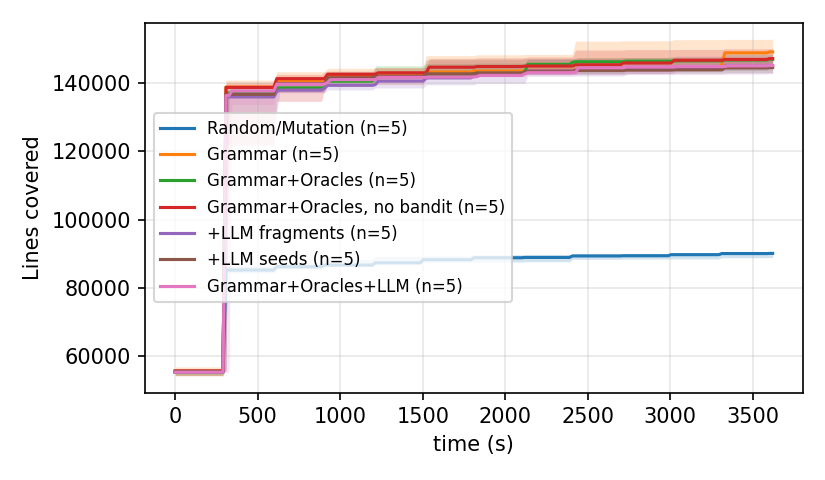
\includegraphics[width=0.44\linewidth]{figures/rq1_lines}
  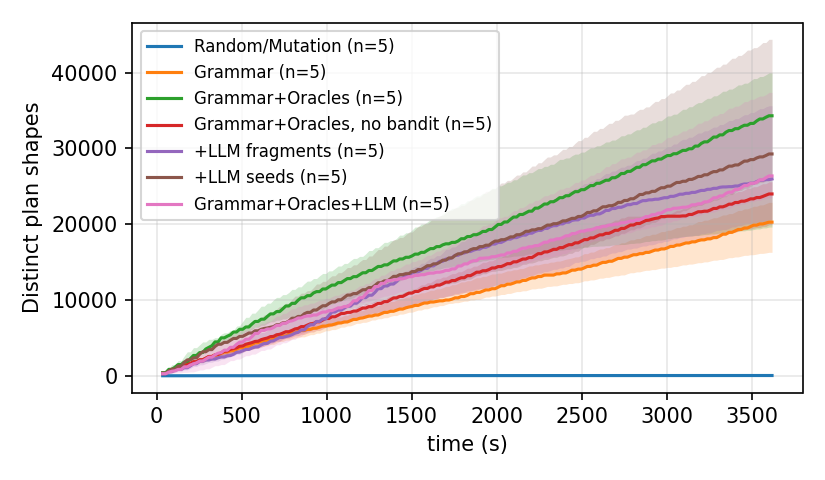
\includegraphics[width=0.44\linewidth]{figures/rq1_plans}
  \caption{\rqref{1}: lines covered (left) and distinct plan shapes (right) over
  time, median and interquartile band of 5 trials per arm.}
  \label{fig:rq1}
\end{figure}

\begin{observation}
\label{obs:grammar}
The typed grammar reaches far more than random mutation: 36.7\% against 22.2\%
of lines ($\hat{A}_{12}=1.00$, $p=0.008$), 101 against 23 SQL features, and
99.3\% against 26.0\% valid statements, although the random arm runs 15 times
more test cases.
\end{observation}

\begin{observation}
\label{obs:oracles-reach}
The oracles do not add line coverage (36.7\% to 36.2\%, $p=0.42$) but they
roughly double the plan shapes (20{,}279 to 34{,}313, $\hat{A}_{12}=0.84$,
$p=0.095$, so with 5 trials this is an effect size, not a significant
difference). The feedback weights contribute: without them the same arm
reaches 23{,}997 plan shapes ($\hat{A}_{12}=0.80$, $p=0.15$), at the price of
validity (96.3\% against 99.4\%, $p=0.016$).
\end{observation}

Oracles also cost throughput: the plan-variant runs and metamorphic checks
lower the statements per second from 67 to 40.

\subsection{\rqref{2}: Bugs and Oracle Precision}
\label{sec:rq2}

Across the \rqref{1} and \rqref{3} campaigns, plus the earlier hunt and smoke
runs, \tool reported 93 distinct bug candidates (after de-duplication by
signature). We triaged all of them (Section~\ref{sec:triage}) and
Table~\ref{tab:rq2} gives the verdicts per oracle.

\begin{table*}[t]
  \centering
  \small
  \caption{\rqref{2}: verdict of every triaged candidate per oracle. Duplicate:
  a real bug that had already been reported upstream. False positives include
  one intended change between versions. Flaky: did not reproduce in three
  re-runs. Open: not decided yet.}
  \label{tab:rq2}
  \begin{tabular}{lrrrrrr}
    \toprule
    Oracle & Candidates & Real & Duplicate & False pos. & Flaky & Open \\
    \midrule
    assertion & 15 & 3 & 10 & 1 & 1 & 0 \\
    crash & 1 & 0 & 0 & 1 & 0 & 0 \\
    cross-version & 25 & 0 & 0 & 7 & 18 & 0 \\
    internal\_error & 4 & 2 & 1 & 0 & 1 & 0 \\
    mm: expr & 3 & 1 & 1 & 1 & 0 & 0 \\
    mm: rls & 5 & 0 & 0 & 5 & 0 & 0 \\
    mm: tlp\_having & 4 & 0 & 0 & 4 & 0 & 0 \\
    mm: tlp\_where & 4 & 1 & 1 & 2 & 0 & 0 \\
    plan-variant & 32 & 1 & 2 & 21 & 8 & 0 \\
    \midrule
    all & 93 & 8 & 15 & 42 & 28 & 0 \\
    \bottomrule
  \end{tabular}

\end{table*}

\paragraph{Bugs.} Table~\ref{tab:bugs} lists the ten bugs we reported. Six
came from running the fuzzer (the campaigns and later runs on newer master builds); four came from
the targeted bug hunt that accompanied them, in which we audited recent planner and executor features with
differential probes. Eight of the ten bugs are fixed upstream, six of them with fixes written by the
authors. The other two are open with our patches. The oracles also found three bugs reported by others days
before us, which we count as duplicates: a wrong result of self-join
elimination under \texttt{ROLLUP} in 18.6 (\#19800, a plan variant), \#19772
(the \texttt{(SELECT e)} rewrite) and \#19784.

\begin{table*}[t]
  \centering
  \footnotesize
  \caption{The ten bugs we reported upstream, the oracle that recognises each,
  and their state on 13~November~2026. All reproduce on the base build
  \texttt{26bd08fb}, which predates the fixes.}
  \label{tab:bugs}
  \begin{tabular}{@{}llll@{}}
    \toprule
    Bug & Report & Oracle & State \\
    \midrule
    \texttt{JSON\_TABLE} assigns no collations & \#19768 & assertion & fixed (our patch) \\
    \texttt{range @> NULL} folded to a constant & \#19793 & \texttt{(SELECT e)} rewrite & reported, patch \\
    \texttt{MERGE}: SubPlan with no parent & \#19802 & internal error & fixed \\
    parallel \texttt{Append} assertion & \#19803 & TLP (\arm{+LLM fragments}) & fixed \\
    \texttt{to\_char(NaN)} breaks \texttt{NORMALIZE} & \#19771 & assertion & fixed (our patch) \\
    \texttt{NOT IN} anti-join ignores a cast & pgsql-bugs & TLP & fixed (our patch) \\
    \texttt{IGNORE NULLS} frame never returns & pgsql-bugs & hang & fixed (our patch) \\
    duplicate statistics expression & pgsql-bugs & assertion & fixed (our patch) \\
    non-finite imported MCV frequencies & pgsql-hackers & CERT estimate & patch \\
    \texttt{corr()} of a constant under partial aggregation & \#19826 & plan variant & fixed (our patch) \\
    \bottomrule
  \end{tabular}
\end{table*}

\paragraph{Rediscovery.} We added each reproducer as a seed that carries its own
check (for a wrong result, the query that must agree), extended the grammar with
what the four hunt bugs need (statistics on expressions, statistics import with
boundary values, a user-defined implicit cast, \texttt{IGNORE NULLS} over
whole-partition frames), and added a \emph{hang} oracle that restarts a server
whose statement outlives its \texttt{statement\_timeout} by ten seconds. One
150-second trial of \arm{Grammar+Oracles} on the base build then reported all
nine bugs reported up to that point, each matched to its catalogue entry, at unchanged validity (99.3\%).
With the tenth reproducer added (\#19826, found by the plan-variant oracle
under partitionwise aggregation), the one-command reproduction, one
150-second trial that replays the seeds in turn, reports all ten bugs.

\begin{observation}
\label{obs:wrong}
Plan-variant and metamorphic oracles found real wrong results in released
versions that no crash oracle can see (BUG~\#19793 and \#19800).
\end{observation}

\paragraph{Precision.} Of the 93 candidates, 28 (30\%) did not reproduce in
three re-runs. Of the 65 others, 8 are real, 15 are duplicates of real bugs and
42 are false positives, so the precision is $8/50=0.16$ without duplicates and
$23/65=0.35$ if duplicates count as true positives. The false positives come
from few classes: six were fixed before the campaigns, and five that the
campaigns revealed were fixed \emph{after} them, tested on the stored
reproducers but not re-measured.
They are equal \texttt{interval} values printed differently depending on
join order (16 candidates; the digest now uses \pg's interval equality),
order-sensitive aggregates sorted by a key that is not the value, such as
\texttt{ORDER BY NULL} (2), state that diverges in the cross-version oracle
after an \texttt{INSERT} only master accepts (5), an RLS rewrite that left a
protected table inside a repeated sub-select unfiltered (5), and an LLM rewrite
that is not an identity (Section~\ref{sec:rq4}). One remaining candidate is
a new bug, which we reported as BUG~\#19826: \texttt{corr()} of a constant input is NULL
serially but 1 under partial aggregation. It is fixed upstream with our patch
(\texttt{ef1b7404}, back-patched to 19).

\subsection{\rqref{3}: Re-injected Bugs}
\label{sec:rq3}

\begin{table*}[t]
  \centering
  \small
  \caption{\rqref{3}: trials (of 5) in which an arm found each re-injected bug,
  with the median time to the first finding. The rows below list, per symptom,
  how many bugs an arm found at all. Only bugs found by some arm have their own
  row; 18 of 20 were found by none.}
  \label{tab:rq3}
  \begin{tabular}{llrrrr}
    \toprule
    Bug & Symptom & \arm{Random} & \arm{Grammar} & \arm{Grammar+Oracles} & \arm{+LLM (both)} \\
    \midrule
    \texttt{11b56ee2} & assertion & 0/5 & 0/5 & 1/5 (2901\,s) & 1/5 (1858\,s) \\
    \texttt{dfcf6fa7} & internal error & 0/5 & 5/5 (458\,s) & 4/5 (509\,s) & 5/5 (1109\,s) \\
    \midrule
    \multicolumn{2}{l}{wrong result, 8 bugs: found} & 0 & 0 & 0 & 0 \\
    \multicolumn{2}{l}{internal error, 5 bugs: found} & 0 & 1 & 1 & 1 \\
    \multicolumn{2}{l}{assertion, 4 bugs: found} & 0 & 0 & 1 & 1 \\
    \multicolumn{2}{l}{missing error, 2 bugs: found} & 0 & 0 & 0 & 0 \\
    \multicolumn{2}{l}{wrong error, 1 bug: found} & 0 & 0 & 0 & 0 \\
    \midrule
    \multicolumn{2}{l}{Bugs found (of 20)} & 0 & 1 & 2 & 2 \\
    \bottomrule
  \end{tabular}

\end{table*}

\begin{observation}
\label{obs:rq3}
With one hour and five trials, the arms found few of the benchmark bugs:
\arm{Random} 0 of 20, \arm{Grammar} 1, \arm{Grammar+Oracles} 2 and \arm{+LLM}
2. No arm found any of the 8 wrong-result bugs.
\end{observation}

The grammar arms found the internal error of fix \texttt{dfcf6fa7} in nearly
every trial (median 458, 509 and 1{,}109 seconds); \arm{Random} never did. The two
arms with oracles also found the assertion of \texttt{11b56ee2}, once each, which
is too little to separate them. The benchmark therefore does \emph{not} show an
advantage of the oracles; that claim rests on \rqref{2}. Three things limit
\rqref{3}: one hour is short for bugs that need a specific combination of
features; attribution is conservative (of the 30 wrong-result failures, 11
reproduce on the fixed server, 19 on no server, and none on a solo server); and
five trials cannot separate arms that find a bug in one trial in five.

\subsection{\rqref{4}: The LLM Extension}
\label{sec:rq4}

The gate accepted 4 of 10 commits (2 in the first round, 2 after repair). Of
the 25 rounds, 16 failed because too few statements ran (mean validity of a
proposal 36.5\%), 4 because the fragment was not derived or did not parse, and
1 on seeds or coverage. The run used 328{,}000 input and 171{,}000 output tokens
at no cost on the free tier.

\begin{observation}
\label{obs:llm}
The LLM arms add SQL features (101 to 104--106, $\hat{A}_{12}=1.00$,
$p=0.004$) but no coverage: lines drop from 36.2\% to 35.7\% ($p=0.42$), plan
shapes from 34{,}313 to 26{,}375, and validity from 96.3\% to 95.3\%.
\end{observation}

It covers only 34 more changed lines over the 10 commits, but the
fragments-only arm found BUG~\#19803: with these models the benefit is modest.

\paragraph{The gate is not enough for rewrites.} All 7 proposed rewrites passed
the gate, but \texttt{NULLIF(\{e\}, NULL::text COLLATE "POSIX")} is not an
identity: it changes the collation, and caused a false positive in \rqref{3}.
Neither the value probe nor the live checks vary the collation; the gate now
rejects an explicit \texttt{COLLATE}. Testing an equivalence on samples is not proof.

\section{Discussion}
\label{sec:discussion}

The results raise a few questions that we want to discuss before turning to
the threats to validity.

\paragraph{Is a larger grammar always better?} Not for a wrong-result fuzzer. A
larger grammar reaches more corner cases of SQL semantics, and some of them
break the assumptions an oracle makes: \texttt{HAVING} without \texttt{GROUP
BY}, \texttt{DISTINCT} over \texttt{numeric} values of different scale, or
\texttt{interval} values that are equal but print differently. The price is paid
in oracle precision, and every rewrite needs a soundness check on the tree.

\paragraph{Why keep the tree?} Mutation re-derives a subtree, the oracles
rewrite one typed node, and reduction replaces a subtree with its smallest
derivation. In each case the generator replays the tree and re-binds names and
types, so the result stays valid SQL. On the \texttt{JSON\_TABLE} bug, tree
reduction followed by token reduction gave a 79-token reproducer, whereas token
reduction alone stopped at 116 tokens. On the tree, a clause is one node with a
known span, which lets \tool apply TLP inside a derived table or a
\texttt{LATERAL} subquery, where a text-based rewrite would have to parse the
query again.

\paragraph{Why compare with the last release?} Plan variants cannot catch a
wrong result that every plan shares, such as a constant that is folded before
any plan is chosen (Figure~\ref{fig:motivating}). The last release does not have
the newest planner rules, so it disagrees exactly on the bugs that new code
introduces. It also disagrees on intended changes, which triage has to
recognise.

\paragraph{Can an LLM be trusted?} Not on its word. A rewrite is a claim about
semantics, and \rqref{4} shows that our gate accepted a wrong one. For
fragments the situation is easier, because the model only has to name SQL that
reaches a commit, and the \gate rejects anything that does not parse, is never
derived, fails on the server or misses the changed lines. Repair rounds helped
only rarely: of the 4 accepted commits, 2 passed in the first round,
and 6 of the 10 commits never passed.

\paragraph{Does the approach carry over to other engines?}
\label{sec:beyond}
After the \pg campaigns we wanted to know whether the same design works beyond
\pg, so we generalized \tool to DuckDB, SQLite, Turso and Apache DataFusion
(branch \texttt{generalized} of our repository). The answer is yes, with a small
adapter per engine. Each engine runs in its own worker process, and a dialect
\emph{overlay} of a few dozen lines drops or rewrites the parts of the \pg
grammar that the engine does not accept. With hand-written overlays, 96.3\% of
the generated queries are valid on DuckDB, 97.7\% on SQLite, 93.3\% on Turso
and 79.4\% on DataFusion. An overlay miner can also draft the overlay from the
measured failure rate of each grammar alternative: one mined round lifted DuckDB
from 32.1\% to 44.1\% valid statements without any line written by hand. Instead of the
\pg plan variants, \tool uses optimizer-rule firing, read from rule switches or
from per-rule plan traces, as feedback and as a coverage measure. We also added rows synthesized with Z3 that make TLP
partitions non-empty, and normalizers learned from probes for cross-engine
comparison; between DuckDB and SQLite, these normalizers reduce held-out
disagreements from 28.7\% to 3.6\%. The engines' own test suites serve as seeds,
and a loop triages new failures and drafts a filing package with a regression
test in the engine's own format.
Finally, \emph{rule kernels}, minimal queries that each make one optimizer rule
fire, are composed in pairs. In 15-minute campaigns (medians of three trials per
arm), they raise the number of distinct optimizer-rule pairs reached from 307 to
386 on DuckDB, from 241 to 276 on DataFusion, and from 86 to 182 on SQLite.
Every kernel trial beat every plain one ($\hat{A}_{12}=1.00$), although three
trials per arm cannot give $p<0.1$.

These campaigns found fourteen bugs. Nine of them were already fixed on the
engine's development branch when we checked. For the other five we filed an
issue and a pull request with a fix and a regression test: Turso \#11594 / PR
\#11595 (\texttt{percentile\_disc} with an expression argument) and \#11796 / PR
\#11797 (an aggregate in \texttt{IN (SELECT ...)} next to a window function,
which gives a spurious error or a panic); DuckDB \#28551 / PR \#28552
(\texttt{min}/\texttt{max} over a nested value computed by a subquery, a 2.0.0
regression), which a maintainer approved for merging and for the 2.0 release
line; DataFusion \#27235 / PR \#27236 (\texttt{UPDATE} and \texttt{DELETE}
statements that repeat an expression fail on an internal common-subexpression
column); and a DataFusion internal error for a scalar subquery inside
\texttt{VALUES}. A single command (\texttt{scripts/reproduce\_generalized.sh})
reproduces all five on the released versions that the campaigns ran on.

\section{Threats to Validity}
\label{sec:threats}

\paragraph{Internal threats.} Every arm runs 5 trials with the same per-trial
seeds on the same build, schema, executor, oracles and budget, each trial has
its own server, a metamorphic mismatch counts only if it repeats, and every
candidate is reproduced three times before triage. But five trials are few:
differences with $p$ above 0.008 are effect sizes, not significant results, and
several conclusions rest on them.

Our own oracles can be wrong. Eleven false-positive classes reached triage, six
before the campaigns and five in them (Section~\ref{sec:rq2}). We fixed the
last five \emph{after} the campaigns and checked them on the stored
reproducers and with unit tests, but did not re-run the campaigns, so the
precision after the fixes is not a measurement. More classes may remain. Verdicts are ours, some made from the reduced reproducer; we
release the reproducers. An accepted LLM rewrite is tested, not proven
(Section~\ref{sec:rq4}). Attribution in \rqref{3} replays on single-bug servers,
so a finding that needs two injected bugs is reported as unattributed.

The two laptops differ, so \rqref{1} and \rqref{3} are not comparable in
absolute throughput; 14 \rqref{1} trials were re-run with the same seeds after a
server failed crash recovery.

\paragraph{External threats.} We test one system at one commit, with one schema
of 9 relations and one set of row-level security policies that we chose;
bugs that need other data shapes, extensions or concurrent sessions are out of
reach. The 23 benchmark bugs are recent fixes with regression tests and may
favour features that recent \pg development touched. The LLM results hold for
free-tier Gemini Flash models on 10 commits; we store every prompt and response.

\paragraph{Construct threats.} Coverage measures what code ran, not whether an
oracle could have seen a bug there. A bug ``found'' in \rqref{3} means a test
case failed on its solo server and passed on the fixed one, even if its symptom
differs from the PoC's. A fragment that passes the \gate reaches the changed
lines; that does not prove it tests the changed behaviour. The rediscovery of
the reported bugs replays their reproducers as seeds: it shows that the
oracles recognise each bug, not that generation alone finds it in a short run.

\section{Related Work}
\label{sec:related}

\paragraph{Metamorphic oracles for database systems.} The work closest to ours
is by Rigger and Su: pivoted query synthesis~\cite{rigger2020pqs},
NoREC~\cite{rigger2020norec} and TLP~\cite{rigger2020tlp}, all implemented in
SQLancer, together with equivalent expression transformation by Jiang and
Su~\cite{jiang2024eet}. These tools have found hundreds of bugs, but they build
the follow-up query from strings produced by their own small generators. We use
the same kinds of oracles, but apply them to typed derivation trees of a grammar
that covers much more of \pg, at any query level, and we report the precision
of each oracle on this larger language.

\paragraph{Guidance for database fuzzing.} Query plan guidance~\cite{ba2023qpg}
steers SQLancer toward new plan shapes, and we use plan shapes in a similar way
as a corpus signal. SQUIRREL~\cite{zhong2020squirrel} mutates an intermediate
representation of SQL with coverage feedback to find crashes, and
SQLRight~\cite{liang2022sqlright} adds the logic-bug oracles of SQLancer to this
setting. CERT~\cite{ba2024cert} checks that a more restrictive query never gets a
larger cardinality estimate, and we include its check. Directed greybox
fuzzing~\cite{bohme2017aflgo} steers a fuzzer toward chosen code locations. We
also direct the campaign toward recent commits, but at the level of SQL features
rather than branches.

\paragraph{Grammar-based and differential SQL testing.} RAGS~\cite{slutz1998rags}
compared the results of several database systems on random SQL, and
SQLsmith~\cite{sqlsmith} generates queries from the catalog of a running \pg.
Instead of comparing different systems, we compare one server with itself under
18 plan variants and with its own last release, which avoids most dialect
differences. We need a typed grammar for this because the oracles must know the
type and the scope of every node.

\paragraph{LLMs for fuzzing.} Fuzz4All~\cite{xia2024fuzz4all} uses an LLM
directly as the input generator. We use the LLM differently: we call it only a
few times per commit, for grammar alternatives and rewrites, and everything it
proposes has to pass a server-side \gate.

\paragraph{Benchmarks, evaluation and reduction.} Magma~\cite{hazimeh2020magma}
ports real bugs into real programs, and Klees et al.~\cite{klees2018evaluating}
showed how fuzzing evaluations go wrong without repeated trials. Following
them, our benchmark reverts real fixes in one server, attributes each finding by
replaying it on single-bug servers, and runs every arm for repeated trials. We
reduce failures with delta debugging~\cite{zeller2002dd} and hierarchical delta
debugging~\cite{misherghi2006hdd}, and we add paired reduction for metamorphic
checks, where the two queries must shrink together to stay equivalent.

\section{Conclusion}
\label{sec:conclusion}

We presented \tool, a fuzzer that generates SQL as typed derivation trees,
rewrites these trees into metamorphic checks, compares each query with its plan
variants and with the last release, and extends its grammar from recent commits
behind a server-side gate. With it we reported ten \pg bugs, eight of which are
fixed upstream, six with our patches. Its grammar reaches 36.7\% of backend
lines against 22.2\% for random mutation, yet in the end it was the precision of
the oracles, not the reach of the generator, that decided how useful the
findings were. We think this is the main thing to improve in future
wrong-result fuzzers: each false-positive class we found came from an oracle
assumption that held for most queries but not for all, so every new rewrite and
every comparison needs its own soundness argument. Finally, with a dialect overlay and a small adapter per engine,
the same core tests DuckDB, SQLite, Turso and DataFusion, where it found five
more bugs that we reported upstream with fixes (Section~\ref{sec:beyond}).

\section*{Data Availability}
\label{sec:data}
Our replication package is the course repository
\url{https://github.com/PASS-IITG/cs5187-term-project-blazing-bhuvi} (MIT
license); the generalized fuzzer of Section~\ref{sec:beyond} is on branch
\texttt{generalized} of the same repository. The \texttt{README.md} lists the
exact dependencies and links every upstream report with its state. It also
gives a one-command reproduction of the headline result
(\texttt{scripts/reproduce.sh}, which finds the ten reported \pg bugs) and one
for the five bugs of the generalized fuzzer
(\texttt{scripts/reproduce\_generalized.sh}). The repository contains the source of \tool with its unit tests,
the grammar and the schema, and the benchmark with the 23 fix commits, their
PoCs and the scripts that build the fixed, solo and injected servers. It also
holds the experiment configurations, the logs and reports of every trial, the
triage verdicts, and the LLM ledger with every prompt and response, so that
\rqref{4} can be replayed without calling the model.

\section*{Use of Generative AI}
\tool calls a large language model as part of its method
(Section~\ref{sec:llm}). In the evaluation this was Google Gemini Flash
(Section~\ref{sec:eval}); every prompt and response, together with the model
that served it, is in the replication package. An AI coding assistant helped
with parts of the implementation and with drafting text. The authors designed
the approach, reviewed all code and text, and checked every statement, citation
and number. All numbers reported here were produced by running the tool and the
scripts.

\section*{Statement of Contributions}
\label{sec:contrib}
Every member of the team can explain every part of the project. The split below
records who did most of the work on each part, and the commit history of the
repository shows the same split (GitHub users \texttt{v28k}, \texttt{Blazing-bhuvi}
and \texttt{doma2542}).

\paragraph{Venu Kummari} Designed and implemented \tool: the typed grammar and
its generator, the metamorphic oracles on derivation trees, the plan-variant,
cross-version, row-level security and cardinality oracles, the executor and the
hang oracle, triage with tree and token reduction, the LLM gate, the re-injected
bug benchmark and the evaluation harness. Reported BUG \#19768
(\texttt{JSON\_TABLE}) and BUG \#19793 (\texttt{range @> NULL}) with patches,
and BUG \#19826 (\texttt{corr()} under partial aggregation), which was fixed
upstream with his patch. Wrote the paper. Built the generalized fuzzer for
DuckDB, SQLite, Turso and DataFusion (Section~\ref{sec:beyond}) and wrote its
five upstream fixes.

\paragraph{Bhuvan Chilukuti} Ran the \rqref{3} campaign on the re-injected bug
benchmark and its attribution, and the cross-version, metamorphic and
audit-driven bug hunts on recent \pg features. Reported, with patches, the
\texttt{NOT IN} anti-join bug, the \texttt{IGNORE NULLS} hang, the duplicate
statistics expression assertion and the non-finite MCV frequencies, and answered
the maintainers on these threads.

\paragraph{Gowtham Reddy} Built the servers, ran the \rqref{1}, \rqref{2} and
\rqref{4} campaigns (35 trials) and wrote their reports, ran the LLM arm with
Gemini Flash over ten commits, and triaged the campaign candidates. Reported BUG
\#19802 (\texttt{MERGE}) and BUG \#19803 (parallel \texttt{Append}), both fixed
upstream, as reporter and tester, and reported BUG \#19771 (\texttt{to\_char})
and wrote its fix, which was committed upstream.

\medskip
\noindent Signed, 13 November 2026:\quad Venu Kummari \quad Bhuvan Chilukuti \quad Gowtham Reddy


\bibliographystyle{ACM-Reference-Format}
\bibliography{references}

\end{document}
